\documentclass[12pt]{article}
\usepackage[margin=1.5cm]{geometry}
\usepackage{parskip}
\usepackage{amsmath}
\usepackage{amssymb}
\usepackage{amsfonts}
\usepackage{enumitem}
\usepackage{graphicx}
\usepackage{stmaryrd}
\graphicspath{ {./images/} }


\begin{document}
\begin{enumerate}[label=(\alph*)]

  \item
    \begin{enumerate}[label=(\roman*)]

      \item
        \begin{enumerate}[label=(\Alph*)]

          \item
            We propose the following microarchitecture:

            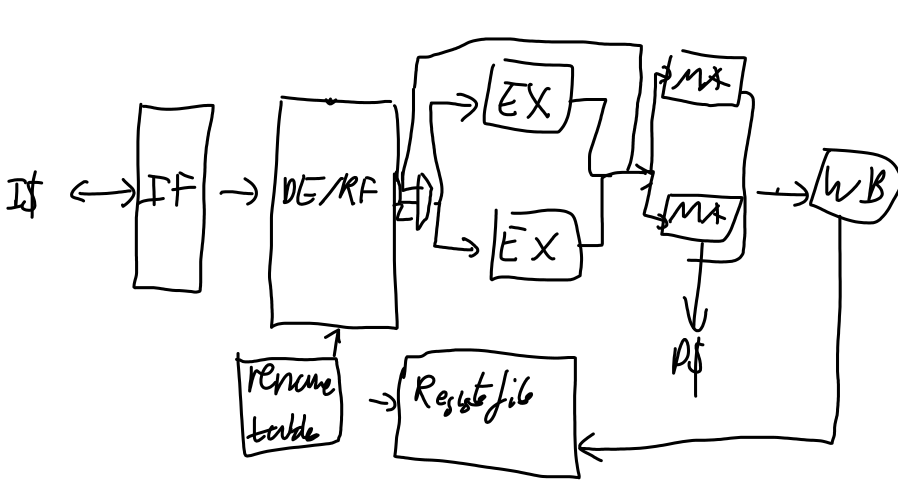
\includegraphics[scale=0.3]{pipeline1}

            Here, we have a traditional 5 stage pipeline, with duplicated execute and memory access stages (since we duplicate all the functional units and the load-store unit).

            The IF stage fetches two instructions from instruction cache, and the DE/RF stage decodes these two instructions, fetching arguments from the register file (using register renaming to avoid name dependencies). It also checks whether or not the two instructions are independent (i.e. there is not a RAW dependency). The execute stages perform ALU/FP operations. The MA stage access memory through the data cache, and the WB stage writes results back to registers. We also have numerous feed-forward paths to prevent stalls where possible.

            \item

              Here, we have a significantly more complex pipeline:

              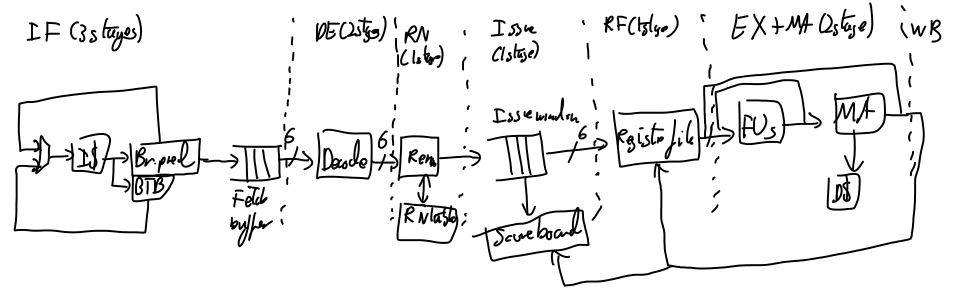
\includegraphics[scale=0.5]{pipeline2}

              Instruction fetch is split into 3 stages, to maintain a high clock frequency and a deep pipeline. Instruction cache feeds into a tournament branch predictor and a BTB, which feed back into the instruction cache for address generation. Then, instructions enter a fetch buffer.

              These are decoded in the decode stage, split into two stages.

              Then, we rename the registers in a single stage (using a register map table) to let us use more physical registers than we have in the ISA, and to remove name dependencies.

              Instructions then enter an issue window/queue, and we use a scoreboard to keep track of when it is safe to actually issue instructions since we permit out-of-order execution.

              Up to 6 instructions are then chosen to be issued, and their operands are read through the register file (having already had the registers renamed).

              Then, we have duplicated functional units and load-store units to permit simultaneous execution. The load-store units access data cache, and might make use of large load and store queues.

              Finally, we write back to the register file in the WB stage, and also update the scoreboard.

            
        \end{enumerate}

        \item
          The large difference in area comes from the significantly more complex issue logic required for out-of-order execution. For example, the branch predictor has to be able to predict on potentially multiple instructions simultaneously within a single clock cycle, and has to provide very good predictions given the depth of the pipeline. This means the area cost is very high.


          Furthermore, we also have to duplicate a lot of logic considering we are scaling up by a factor of 3. We will probably have many ALUs and load-store units, as well as enough area for large load-store queues. For this many instructions, we will likely also have many more physical registers to avoid false dependencies where possible, which also takes up a lot of area.
    \end{enumerate}

    \item
      A simple BTB design will simply associate a branch's pc along with its target, i.e. where it branched to list (if it was taken).

      Indirect branches can have multiple targets, so if the branch target changes for the same branch address, then we will predict the wrong branch target, even if the branch is taken both times.

      \item
        If we favour a particular branch target, we ought to predict this branch target over others, even if for a single time we switch to another branch target. Therefore, we might optimise our BTB design to also contain a small saturating counter that begins at the half way point. When we predict the target correctly, we increment the counter, and decrement the counter if not. If we incorrectly predict the target and the counter's MSB is 0, then we can swap out the branch target.


        
\end{enumerate}
\end{document}
